%----------------------------------------------------------------------------------------
%	DOCUMENT CONFIGURATIONS
%----------------------------------------------------------------------------------------
\documentclass[a4paper, 14pt]{extarticle}
\usepackage{Styles/style}
\usepackage{listings}
\usepackage[utf8]{inputenc}
\usepackage[russian]{babel}
\usepackage{Styles/Personal_data}
\usepackage[T1]{fontenc}
\usepackage{float}
\usepackage{longtable}
\lstset{inputencoding=utf8,
   extendedchars=false,
   %         stringstyle=\usefont{T2A}{fcr}{b}{n},
   language=C++, %Язык по умолчанию Code langugage
   belowcaptionskip=5pt,
   basicstyle=\usefont{T2A}{fcr}{m}{n}\footnotesize,                   % Code font, Examples: \footnotesize, \ttfamily
   % keywordstyle=\color{OliveGreen},      % Keywords font ('*' = uppercase)
   commentstyle=\color{gray},              % Comments font
   keywordstyle=\usefont{T2A}{fcr}{b}{n},  % Keywords font ('*' = uppercase)
   % commentstyle=\usefont{T2A}{fcr}{m}{sl},              % Comments font
   numbers=left,                           % Line nums position
   numberstyle=\tiny,                      % Line-numbers fonts
   stepnumber=1,                           % Step between two line-numbers
   numbersep=5pt,                          % How far are line-numbers from code
   % backgroundcolor=\color{lightlightgray}, % Choose background color
   frame=none,                             % A frame around the code
   tabsize=2,                              % Default tab size
   captionpos=b,                           % Caption-position = bottom
   breaklines=true,                        % Automatic line breaking?
   breakatwhitespace=true,                 % Automatic breaks only at whitespace?
   showspaces=false,                       % Dont make spaces visible
   showtabs=false,                         % Dont make tabls visible
   columns=flexible,                       % Column format
   morekeywords={__global__, __device__},  % CUDA specific keywords
   keepspaces = true   %!!!! пробелы в комментариях
}
\newcommand{\fig}[2]{
\begin{figure}[H]	
	\begin{center}
		\includegraphics[scale=1]{Images/#1.png}
\caption{#2}
	\label{#1}
	\end{center}
\end{figure}
}
\newcommand{\blockschema}[2]{
\begin{figure}[H]	
	\begin{center}
		\includegraphics[width=\textwidth]{Images/#1.png}
\caption{#2}
	\label{#1}
	\end{center}
\end{figure}
}

\usepackage{etoolbox}

\newcounter{totfigures}
\newcounter{tottables}
\newcounter{totpages}

\providecommand\totfig{}
\providecommand\tottab{}
\providecommand\totpage{}

\makeatletter
\AtEndDocument{
  \addtocounter{totfigures}{\value{figure}}
  \addtocounter{totfigures}{-1}
  
  \addtocounter{tottables}{\value{table}}
  \addtocounter{tottables}{-1}
  
  \addtocounter{totpages}{\value{page}}
  \addtocounter{totpages}{-1}
  
  \immediate\write\@mainaux{
    \string\gdef\string\totfig{\number\value{totfigures}}
    \string\gdef\string\tottab{\number\value{tottables}}
    \string\gdef\string\totpage{\number\value{totpages}}
  }
}
\makeatother

\usepackage{totcount}
\newtotcounter{citnum} %From the package documentation
\def\oldbibitem{} \let\oldbibitem=\cite
\def\cite{\stepcounter{citnum}\oldbibitem}



\addbibresource{Bibliography/references.bib} % библиографическая база данных

\begin{document}

%----------------------------------------------------------------------------------------
%	TITLE PAGE
%----------------------------------------------------------------------------------------

%\def\data_dopuska{01.06.2018 г.} % Дата допуска работы к защите

\begin{titlepage}
\begin{spacing}{1.075}
\center 

\normalsize \textbf{Липецкий государственный технический университет}\\

\vspace{0.5 cm}

\normalsize 
Факультет автоматизации и информатики \\
Кафедра прикладной математики\\

\vspace{1.5 cm}

\normalsize 	ВЫПУСКНАЯ КВАЛИФИКАЦИОННАЯ\\
РАБОТА БАКАЛАВРА\\
по направлению \major \\
тип программы  Академическая \\
профиль \profil

\vspace{1 cm}

\MakeUppercase{\thema}

\vspace*{1.5 cm}

\normalsize
\begin{spacing}{1.0}
\begin{tabular}{b{4.75cm} p{1cm} c p{1cm} c}
Студент  	&   &  &  &  \student \\ \hhline{~~-~-} 

 	&  & \footnotesize \hspace{0.5cm} подпись, дата	\hspace{0.5cm} &  & \footnotesize  фамилия, инициалы \\ [-0.4cm]
Группа \underline{\group}  	&   &  &  &  \\ [0.2cm]
Руководитель  	&   &  &  &  \\
\centering{\ad}	&   &  &  & \adviser \\ \hhline{-~-~-} 
\footnotesize учёная степень, учёное звание	 	&  	& \footnotesize \hspace{0.5cm} подпись, дата	\hspace{0.5cm} &  & \footnotesize  фамилия, инициалы \\ [0.2cm]

\textbf{Нормоконтроль}  	&   &  &  &  \\
\multicolumn{2}{l}{программного обеспечения}    &  &  & \normalsize Сысоев А.С. \\ \hhline{~~-~-} \footnotesize  	&  	& \footnotesize \hspace{0.5cm} подпись, дата	\hspace{0.5cm} &  & \footnotesize  фамилия, инициалы \\ [0.2cm]


\multicolumn{2}{l}{оформления работы}    &  &  & \normalsize Сысоев А.С. \\  \hhline{~~-~-} \footnotesize  	&  	& \footnotesize \hspace{0.5cm} подпись, дата	\hspace{0.5cm} &  & \footnotesize  фамилия, инициалы \\ [0.2cm]

\vspace{0.2cm}  
Рецензент  	&   &  &  &  \\
\centering{\small \rd}	&   &  &  & \recenzent \\ \hhline{-~-~-} 
\centering{\footnotesize уч. ст., уч. зв., должность}	 	&  	& \footnotesize \hspace{0.5cm} подпись, дата	\hspace{0.5cm} &  & \footnotesize  фамилия, инициалы \\ [0.3cm]
\multicolumn{5}{l}{\textbf{Работа рассмотрена кафедрой и допущена к защите в ГЭК}}  \\ [0.3cm]
Зав. кафедрой	&   &  &  & Галкин А.В. \\ \hhline{~~-~~} 
				&   &  &  & \data_dopuska \\ 
 

\end{tabular} 



\end{spacing}




\vspace*{1.5cm}
\normalsize
\centering Липецк 2018 г.

\end{spacing}

\end{titlepage}  % если есть программа
%\def\data_dopuska{01.06.2018 г.} % Дата допуска работы к защите

\begin{titlepage}
\begin{spacing}{1.075}
\center 

\normalsize \textbf{Липецкий государственный технический университет}\\

\vspace{0.5 cm}

\normalsize 
Факультет автоматизации и информатики \\
Кафедра прикладной математики\\

\vspace{1.5 cm}

\normalsize 	ВЫПУСКНАЯ КВАЛИФИКАЦИОННАЯ\\
РАБОТА БАКАЛАВРА\\
по направлению \major \\
тип программы  Академическая \\
профиль \profil

\vspace{1 cm}

\MakeUppercase{\thema}

\vspace*{1.5 cm}

\normalsize
\begin{spacing}{1.0}
\begin{tabular}{b{4.75cm} p{1cm} c p{1cm} c}
Студент  	&   &  &  &  \student \\ \hhline{~~-~-} 

 	&  & \footnotesize \hspace{0.5cm} подпись, дата	\hspace{0.5cm} &  & \footnotesize  фамилия, инициалы \\ [-0.4cm]
Группа \underline{\group}  	&   &  &  &  \\ [0.2cm]
Руководитель  	&   &  &  &  \\
\centering{\ad}	&   &  &  & \adviser \\ \hhline{-~-~-} 
\footnotesize учёная степень, учёное звание	 	&  	& \footnotesize \hspace{0.5cm} подпись, дата	\hspace{0.5cm} &  & \footnotesize  фамилия, инициалы \\ [0.2cm]

\textbf{Нормоконтроль}  	&   &  &  &  \\

\multicolumn{2}{l}{оформления работы}    &  &  & \normalsize Сысоев А.С. \\  \hhline{~~-~-} \footnotesize  	&  	& \footnotesize \hspace{0.5cm} подпись, дата	\hspace{0.5cm} &  & \footnotesize  фамилия, инициалы \\ [0.2cm]

\vspace{0.2cm}  
Рецензент  	&   &  &  &  \\
\centering{\small \rd}	&   &  &  & \recenzent \\ \hhline{-~-~-} 
\centering{\footnotesize уч. ст., уч. зв., должность}	 	&  	& \footnotesize \hspace{0.5cm} подпись, дата	\hspace{0.5cm} &  & \footnotesize  фамилия, инициалы \\ [0.3cm]
\multicolumn{5}{l}{\textbf{Работа рассмотрена кафедрой и допущена к защите в ГЭК}}  \\ [0.3cm]
Зав. кафедрой	&   &  &  & Галкин А.В. \\ \hhline{~~-~~} 
				&   &  &  & \data_dopuska \\ 
 

\end{tabular} 



\end{spacing}




\vspace*{2.5cm}
\normalsize
\centering Липецк 2018 г.

\end{spacing}

\end{titlepage} % если нет программы

%----------------------------------------------------------------------------------------
%	TASK
%----------------------------------------------------------------------------------------

%\def\datavydachi{25.12.2017 г.} % Дата выдачи задания
\def\datavydachiPr{<<25>> декабря 2017 г.} % Дата выдачи задания (МЕСЯЦ-ПРОПИСЬЮ)
\def\datasdachi{25.05.2018 г.} % Дата сдачи работы руководителю
\def\datadopuska{01.06.2018 г.} % Дата допуска работы к защите


\pagestyle{empty}
\normalsize
\begin{center}
	\textbf{Липецкий государственный технический университет}
\end{center}

\noindent
\begin{tabular}{p{6cm} p{1cm} c p{1cm} c}
	\textbf{Факультет} ФАИ  &   &  &  & \textbf{Зав. кафедрой} \underline{Галкин А.В.}   \\ \hhline {~~~~~}
	\textbf{Кафедра} ПМ  &   &  &  & \underline{\hspace{2.5cm}\datavydachiPr}  \\ \hhline {~~~~~}
\end{tabular}

\begin{center}
	\textbf{ЗАДАНИЕ НА ВЫПОЛНЕНИЕ \\ ВЫПУСКНОЙ КВАЛИФИКАЦИОННОЙ РАБОТЫ}
\end{center} 

\noindent
\textbf{Студенту} \hspace{0.25cm} \studentDat \hspace{0.25cm} \textbf{группы} \group \\

\noindent


\begin{enumerate}
	\item \textbf{Тема} \thema
	
%=============== ТОЛЬКО ЗДЕСЬ НАДО ЧТО-ТО ИСПРАВЛЯТЬ =====================
	
	\item \textbf{Исходные данные} Физические свойства металла рабочих валков и прокатной полосы.
	
	\item \textbf{Ожидаемые результаты} Распределение температуры в очаге деформации в процессе горячей прокатки.
	
	\item \textbf{Срок сдачи работы руководителю} \hspace{1cm} \datasdachi
	
%=========================================================================
		
	\item \textbf{Дата выдачи задания} \hspace{1cm}  \datavydachi
	
	\item \textbf{Руководитель работы}
		\begin{flushright}
			\underline{\hspace{4cm}} /\adviser/
		\end{flushright}
		
	\item \textbf{Задание принял к исполнению студент}
		\begin{flushright}
			\underline{\hspace{4cm}} /\student/
		\end{flushright}	
\end{enumerate}			
	
	

%----------------------------------------------------------------------------------------
%	ABSTRACT
%----------------------------------------------------------------------------------------

%\newpage
\pagestyle{plain}
\setcounter{page}{3}
\section*{АННОТАЦИЯ}

Аннотация отражает основное содержание работы. В аннотации излагают сведения о работе, достаточные для принятия решения о целесообразности обращения к первичному документу. Объем аннотации -- не более одной страницы.

Аннотацию строят по следующей схеме:
\begin{itemize} 
\item выходные сведения об объеме работы, а также количестве иллюстраций, таблиц, источников в списке литературы, приложений, например:

С. 80. Ил. 8. Табл. 16. Литература 32 назв. Прил. 2;

\item текст аннотации, содержащий основную часть, отражающую сущность выполненной работы и краткие выводы, в том числе о возможности применения полученных результатов на производстве и в учебном процессе;
\item перечень слайдов для работ, содержащих графическую часть, например:
\end{itemize}

\begin{table}[h]

\begin{tabular}{p{14.5cm} p{1cm}}
\multicolumn{2}{c}{ГРАФИЧЕСКАЯ ЧАСТЬ} \\
	Слайд 1. Цель и задачи исследования  & 1 \\
	Слайды 2-3. Подходы к вычислению...  & 2 \\
	Слайд 4. Пример & 1 \\
\hline
	Всего слайдов & 10
\end{tabular}

\end{table} 


%----------------------------------------------------------------------------------------
%	CONTENTS
%----------------------------------------------------------------------------------------

%\renewcommand\contentsname{\centering Оглавление}

\tableofcontents 

\newpage 


%----------------------------------------------------------------------------------------
%	INTRODUCTION
%----------------------------------------------------------------------------------------

%\section*{Введение}
\addcontentsline{toc}{section}{Введение}

На металлургических предприятиях, в частности ПАО <<НЛМК>>, стоит проблема разработки новых технологий для горячей прокатки металла. Связано это с тем, что на данный момент нет средства для того, чтобы модельно проэкспериментировать с различными настройками оборудования и приходится разрабатывать новые методы прокатки эмпирически. Очевидно, при неудачных попытках огромное количество металла уходит на утилизацию. 

Чтобы избежать колоссальных материальных потерь, необходим способ, при котором можно было бы моделировать поведение физических свойств материалов и заранее определять настройки оборудования, при которых в результате прокатки не получится бракованная партия, а значит минимизировать потенциальные потери. Потери также большие из-за того, что часто необходимо не создавать, а оптимизировать существующие методы прокатки. Не сделав это, можно потерять довольно большое количество денег из-за низкой цены, которая в свою очередь будет зависеть от качества конечного продукта. К тому же можно потерять клиентуру, которая из-за слишком низкого качества металла начнет обращаться к другим поставщикам, даже несмотря на то, что они могут находится далеко и будут появляться дополнительные издержки от транспортировки в жертву лучшего качества.

В данной работе предлагается такой способ, а именно программное обеспечение, рассчитывающее физические характеристики процесса прокатки. С его помощью оператор может оценить износ материалов при различных настройках оборудования. Так же информация, выводимая представленным ПО, полезна при оценке качества конечного продукта, что может способствовать более высокой его цене на рынке.

\textbf{Цель} - разработать программное обеспечение, способное прогнозировать температурный режим на рабочих валках и полосе стали при горячей прокатке.

В соответствии с целью исследования были поставлены следующие \textbf{задачи:}
	\begin{itemize}
		\item изучить литературу, описывающую процесс горячей прокатки;
		\item изучить свойства материалов, из которых сделаны рабочие валки и прокатная сталь;
		\item разработать математическую модель, описывающую распределение температуры в глубину валка и полосы;
		\item исследовать зависимости различных физических свойств материалов от температуры.
   	\end{itemize}
\newpage


%----------------------------------------------------------------------------------------
%	MAIN PART
%----------------------------------------------------------------------------------------

%\newpage

\section{Обзор процесса горячей прокатки и постановка задачи} 

\subsection{Процесс горячей прокатки}

Процесс пластической деформации металла между двумя или несколькими вращающимися рабочими валками называется прокаткой \cite{Tselikov}.

Прокатка осуществляется разными способами, которые различаются:
\begin{itemize}
\item направлением обработки (продольная, поперечная и винтовая
прокатка);
\item режимом работы станов (непрерывная и реверсивная прокатка);
\item состоянием металла (горячая, теплая, холодная прокатка);
\item формой изделия (лист, сплошной или пустотелый профиль).
\end{itemize}

Рабочие валки могут быть с гладкой бочкой или с нарезанными калибрами. Если оси валков параллельны и лежат в одной плоскости, валки имеют одинаковые диаметры и вращаются в разные стороны с одинаковыми окружными скоростями, прокатываемый металл однороден по своим механическим свойствам и на него действуют только силы от валков, то такой процесс прокатки называется \textit{простым}.

Пространство, ограниченное сверху и снизу дугами захвата (рис. 1), боковыми гранями полосы и плоскостями входа и выхода металла из валков, называется \textit{геометрическим очагом (зоной) деформации} (рис. 2).

\blockschema{2}{Схема очага деформации при прокатке}

\textit{Фактический очаг} деформации больше геометрического и включает в себя внеконтактные зоны, а также \textit{зоны упругой деформации}.

Разность  вцысот полосы при входе и выходе из валков называют \textit{абсолютным обжатием}: $\Delta h = h_0 - h_1$, разность между конечной и начально шириной полосы - \textit{уширением}: $\Delta B = B_1 - B_0$.

Дугу, по которой валок соприкасается с металлом, называют дугой захвата, а горизонтальную проекцию этой дуги $l$ принимают за длину геометрического очага деформации.

\textit{Углом захвата} $\alpha$ называют центральный угол, соответствующий дуге захвата, и находят по уравнению $$\cos \alpha = 1 - \frac{\Delta h}{D}.$$

При небольших углах захвата ($\alpha = 10 - 15^\circ$) можно считать, что $\alpha \approx \sin \alpha$, и тогда $$\alpha \approx \sqrt{\frac{\Delta h}{R}}.$$

\fig{3}{Схема очага деформации при прокатке с обозначениями}

\subsection{Технология производства ПАО <<НЛМК>>}

Новолипецкий металлургический комбинат является предприятием с полным металлургическим циклом, а это значит, что на промышленной площадке комбината располагаются все производства, необходимые для того, чтобы железная руда, пройдя все технологические этапы, превратилась в конечный металлургический продукт – холоднокатаный прокат, в том числе с покрытиями.
Общая схема производства включает следующие переделы: 

\begin{itemize}
\item Агломерационное производство с четырьмя агломашинами;
\item Коксохимическое производство с четырьмя батареями, оборудованными установками беспылевой выдачи кокса;
\item Доменное производство, представленное двумя доменными цехами с шестью доменными печами;
\item Сталеплавильное производство, представленное двумя конвертерными цехами, в состав которых входят шесть конвертеров и девять УНРС.
\item Прокатное производство, представленное цехом горячего проката с непрерывным широкополосным станом горячей прокатки 2000 и тремя цехами холодной прокатки, в состав которых входят два двадцативалковых стана, два реверсивных стана, один непрерывный стан, три дрессировочных стана, один полностью непрерывный стан <<бесконечной прокатки>>.
\end{itemize}

\blockschema{17}{Схема производства металла на ПАО <<НЛМК>>}

Прокатное производство представлено производством горячего проката (ПГП), производством холодного проката и покрытий (ПХПП), производством трансформаторной стали (ПТС) и производством динамной стали (ПДС). Сталь, прокатанная на стане <<2000>> ПГП (горячекатаный прокат), является товарной продукцией НЛМК третьего передела и служит заготовкой в производстве холоднокатаного проката. Тем важнее минимизировать издержки производства.

Производство горячекатаного проката на комбинате осуществляется на непрерывном широкополосном стане (НШС) <<2000>>. Производительность стана – около 5 млн 780 тысяч тонн проката в год. Длина технологической линии производства стальной горячекатаной полосы – 1,2 километра. Стан оснащен новейшими системами автомати-ческого управления, приводами всех основных механизмов, а также системами регули-рования и управления технологическим процессом.

На отводящем рольганге расположена автоматизированная система контроля качества поверхности полосы. На стане производят прокат толщиной 1,45-25,00 мм и шириной 900-1850 мм:

\begin{itemize}
\item товарный прокат из углеродистой и низколегированной стали на внутренний рынок и на экспорт;
\item прокат для дальнейшей холодной прокатки в ПХПП и ПДС (подкат) из углеродистой и низкоуглеродистой стали;
\item прокат из электротехнических марок стали (динамной и трансформаторной) для дальнейшей холодной прокатки в ПТС и ПДС.
\end{itemize}

Горячая прокатка начинается с предварительного разогрева слябов в методических нагревательных печах стана до температуры $1200-1250^\circ$С в течение 3–4 часов. Участок нагревательных печей имеет в своем составе пять нагревательных печей: две толкательные и три новые с шагающими балками. Нагрев в новых печах производится от математической модели. Печи отапливаются смешанным природно-доменным газом. Затем разогретые слябы выдаются на рольганг стана и транспортируются к черновой группе клетей. Черновая группа клетей состоит из:

\begin{itemize}
\item чернового вертикального окалиноломателя, который при помощи двух вертикально расположенных валков разрушает окалину с поверхности сляба;
\item реверсивной двухвалковой клети № 1;
\item четырех последовательно расположенных универсальных четырехвалковых клетей № 2–5.
\end{itemize}

\fig{18}{Универсальная четырехвалковая клеть черновой группы}

В черновой группе сляб проходит, так называемую, черновую (начальную) обработку, прокатываясь последовательно в каждой клети до нужной промежуточной толщины, в зависимости от конечной толщины проката. Для удаления окалины в линии стана установлены специальные приспособления (гидросбивы), которые струей воды (давлением 12,0–16,0 МПа) очищают поверхность металла. Из черновой группы клетей прокат (раскат) транспортируется по промежуточному рольгангу к чистовой группе клетей.

Чистовая группа стана состоит из:

\begin{itemize}
\item летучих ножниц для обрезки переднего и заднего концов раската;
\item чистового двухвалкового окалиноломателя для разрушения окалины, которая образуется при окислении металла на воздухе во время транспортировки раската по промежуточному рольгангу;
\item семи последовательно расположенных четырехвалковых клетей.
\end{itemize}

Все клети чистовой группы оборудованы гидронажимными устройствами. Клети № 7-12 оснащены современными устройствами осевой сдвижки и системой противоизгиба рабочих валков для регулирования поперечной разнотолщинности прокатываемых полос. В чистовой группе клетей производят чистовую, или, другими словами, окончательную прокатку до конечной (заданной) толщины полосы. После выхода из последней клети стана полоса транспортируется по отводящему рольгангу, где для обеспечения необходимых механических свойств металла и соблюдения температурного режима смотки охлаждается водой из установки ускоренного охлаждения (душирования) полосы, и далее сматывается в рулоны на моталках (3 гидравлические моталки).

\fig{19}{Чистовая группа клетей стана <<2000>>}

Смотанные рулоны обвязывают по образующей на автоматизированных машинах обвязки и в зависимости от назначения, по конвейеру направляют:
\begin{itemize}
\item в отделочное отделение для обработки или порезки на листы (полосы) на агрегатах резки с последующей отгрузкой потребителям – товарный прокат;
\item в отделочное отделение для последующей отгрузки железнодорожным транспортом в ПТС и ПДС – подкат для дальнейшей холодной прокатки;
\item в ПХПП – подкат для дальнейшей обработки.
\end{itemize}

\subsection{Постановка задачи}

В условиях невозможности модельно узнать энергосиловые и температурные значения в процессе горячей прокатки в очаге деформации, большое количество материала используется не для готового продукта, а лишь для тестов. Поэтому необходимо разработать программу, способную рассчитывать нужные характеристики исходя из параметров прокатки.

Необходимо, как результат, получить значение в зоне очага деформации следующих характеристик:
\begin{itemize}
\item величину теплового потока;
\item нормальное давление, оказываемое на полосу;
\item сопротивление деформации;
\item касательное давление и предел текучести;
\item распределение температуры.
\end{itemize}

\newpage
%\section{Математическая модель процесса, оптимизация процесса, управление процессом}

\subsection{Первичный обзор задачи}
Рассматривается задача о распределении температур в системе валок-полоса в очаге деформации при горячей прокатке.

Так как задача симметрична, можно рассматривать только верхнюю часть очага. Система представляется следующим образом: рассчитывается распределение температуры в стержне (верхняя часть – валок, нижняя - полоса), который со временем перемещается по области очага (рис. 3). Это позволяет упростить уравнение до одной пространственной переменной. Получается, что рассматривается функция $u(x, t)$. Где $x$ - единственная пространственная координата, а $t$ - это время, в течение которого стержень перемещается по области.

Из-за круглой формы валка и также из-за того, что толщина полосы со временем изменяется, задача будет рассматриваться в полярных координатах. Тогда функция будет зависеть от расстояния от центра координат(радиуса) и от угла: $u(r, \varphi)$.

\fig{4}{Схема очага деформации в полярных координатах}
Условно, всю эту область можно разделить на 2 части. На рисунке они отделены друг от друга линией, обозначенной буквой $R$.

\subsection{Непрерывная модель}

Математическое моделирование процесса осуществляется в несколько этапов: сначала строятся дифференциальные модели, которые аппроксимируются конечно-разностными, затем
для каждого очага деформации по входным усилиям адаптируются коэффициенты
трения. Модели, полученные в результате такого ремоделирования (замены исходных моделей), используются для расчета искомых величин.

Для начала рассмотрим геометрию процесса.

Пусть $R$ - радиус валка, $h_b$ - толщина полосы на входе в очаг и $h_a$ - толщина полосы на выходе из очага, $\Delta h = h_b - h_a$ - разница толщин полосы, тогда

длина очага (рис. 3 отрезок $DG$)
$$L = \sqrt{\Delta h R - \frac{\Delta h^2}{4}};$$

угол в полярных координатах между началом и концом очага, а также правая граница по координате $\varphi$ (рис. 3 $\angle CAB$)  
$$\varphi_{max} = \arcsin\Bigl(\frac{L}{R}\Bigr);$$

величина угла во второй части очага (рис. 3 $\angle CAD$) 
$$\alpha = \arctan\Bigl(\frac{L}{R + \frac{h_a}{2}}\Bigr),$$ 
тогда величина угла в первой части (рис. 3 $\angle DAB$) 
$$\beta = \varphi_{max} - \alpha.$$

В полярных координатах граница для радиуса будет меняться.
$$
r_{max}(\varphi) = 
\begin{cases} 
\cfrac{L}{\sin(\varphi_{max} - \varphi)} \text{, при } \varphi \in [0; \beta]
 \\ 
\cfrac{R + \frac{h_a}{2}}{\cos(\varphi_{max} - \varphi)} \text{, при } \varphi \in [\beta; \varphi_{max}].
\end{cases} 
$$

Вся зона очага делится на 3 зоны (рис. 4). Зона отставания (по дуге СL), зона прилипания (по дуге LM) и зона опережения (по дуге MB). Возникают они потому что, полоса во время контакта имеет непостоянную скорость из-за изменения своей толщины и получается так, что в зоне отставания скорость вращения валка больше скорости проката полосы, а в зоне опережения наоборот, полоса достигает скорости, большей, чем скорость вращения валка. В зоне прилипания же есть единственная точка, в которой скорость валка и скорость полосы совпадают полностью. Опережение и отставание имеют большое значение при расчете непрерывных станов не только в отношении режимов обжатий и скоростей, но также при определении усилий и моментов прокатки, усилий натяжения полосы между клетями стана \cite{process_prokatki}.

\fig{5}{Разделение на зоны}
Нормальное напряжение $p_{contact}$ в очаге деформации рассчитывается по формуле 
\begin{equation}
p_{contact}(\varphi) = \min_{\varphi \in [0; \varphi_{max}]}{(p_{back}(\varphi); p_{forw}(\varphi))},
\end{equation}

где напряжения $p_{back}$ и $p_{forw}$ - нормальные напряжения в зоне отставания и опережения, соответственно, и удовлетворяют уравнениям равновесия Т.Кармана
\begin{equation}
dp_{back} = (K_c - \frac{\mu p_{back}}{\tan \varphi})\frac{dh}{h},
\label{p_back}
\end{equation}

\begin{equation}
dp_{forw} = (K_c + \frac{\mu p_{forw}}{\tan \varphi})\frac{dh}{h}.
\label{p_forw}
\end{equation}

Здесь $K_c$ — сопротивление деформации полосы; $\mu$ - коэффициент трения; $\varphi$ — угол между касательной к поверхности валка и горизонтальной плоскостью; $h=h(\varphi)$ - функция, описывающая изменение толщины полосы в очаге. Для определения сопротивления деформации $K_c$ полосы используется формула
\begin{equation}
K_c = S \cdot \sigma_{\text{о.д.}} \cdot u_i^{a} \cdot (10 \cdot \varepsilon_i)^b \cdot \Bigl(\frac{T_i}{1000}\Bigr)^c;
\label{K_c}
\end{equation}

где $S, a, b, c$ - постоянные, определяемые для каждой марки стали по результатам испытания на пластометре;

$u_i$ - скорость деформации в клети на $i$-том очаге;

$\varepsilon_i$ - относительное точечное обжатие на $i$-том очаге;

$T_i$ - температура полосы на выходе из $i$-того очага.

$\sigma_{\text{о.д.}}$ - базисное сопротивление деформации, определенное при параметрах $T = 1000^oC$, $\varepsilon = 0.1$, $u = 10 c^{-1}$ \cite{disser_pospelov}.

Также существуют модели для расчетов параметров $S, a, b, c$ в зависимости от химического состава стали. Эти модели более точные, т.к. химический состав стали одной и той же марки может быть различным, а также потому что в справочных материалах может не быть значений этих коэффициентов для новых марок стали.

Нам понадобится также информация о нейтральном сечении, то есть о точке с координатами $(R, \varphi^*)$ - пересечения решений уравнений (\ref{p_back}) и (\ref{p_forw}), и толщине $h_{neutr} = h (\varphi^*)$ в нейтральном сечении.

Значение коэффициента трения $\mu$ для каждого очага деформации определяется обратным пересчетом по фактическому усилию прокатки. А именно, на каждом очаге задается начальное приближение $\mu_0$ для коэффициента трения. После расчета контактного напряжения $p_{contact}$ определяется расчетное усилие прокатки $F$ как
суммарное давление по площади контакта:
$$F=W \int^L_0 p_{contact}(\varphi)d\varphi,$$

где $W$ — ширина полосы. Затем расчетное значение усилия сравнивается с фактическим, и коэффициент трения корректируется.

Скорость относительного скольжения $\omega_{slip}$ поверхностей валка и полосы вычисляется по формуле 
$$w_{slip}(\varphi) = \Bigl|V\cdot \Bigl(\frac{h_{neutr}}{h(\varphi)} - 1\Bigr)\Bigr|,$$
 где $V$ — скорость полосы
в очаге. 

Касательные напряжения определяются выражением 
\begin{equation}
\tau_{cont}(\varphi) = \mu  p_{contact}(\varphi),
\end{equation}
а предел текучести
\begin{equation}
\tau_{yield}(\varphi) = \frac{K_c(\varphi)}{1.15 \cdot 2},
\end{equation}

Для расчета плотности теплового потока $q$, генерируемого трением в зоне контакта
используется формула 
\begin{equation}
q(\varphi) = \tau(\varphi)\cdot \omega_{slip}(\varphi),
\end{equation}

где 
$$
\tau(\varphi) = 
\begin{cases} 
\min{(\tau_{cont}(\varphi);\tau_{yield}(\varphi))} \text{, при } \varphi \in [0; \varphi^*]
 \\ 
-\min{(\tau_{cont}(\varphi);\tau_{yield}(\varphi))} \text{, при } \varphi \in [\varphi^*; \varphi_{max}].
\end{cases} 
$$

Прирост температуры полосы в сечении $\varphi$ от пластической деформации задается формулой 
$$\Delta T_{def} = \frac{\eta}{c_S \rho_S} K_c \ln \frac{h(\varphi)}{h(\varphi - \Delta \varphi)},$$ 
где $\eta$ = 0,85 — коэффициент выходного потока тепла от пластической деформации; $c_S$ — удельная теплоемкость полосы; $\rho_S$ — плотность полосы.

Распределение температур подчиняется уравнению теплопроводности. Необходимо еще учитывать факт того, что при горячей прокатке на полосе прокатной стали образуется окалина. Таким образом, необходимо решить систему из трех уравнений (для валка, для окалины и для полосы) с краевыми условиями первого и второго рода.

В общем виде уравнение для функции $u(r, t)$ выглядит следующим образом

$$\frac{\partial u}{\partial t} - a \frac{\partial^2u}{\partial r^2} = f(r, t).$$

Так как вместо времени мы рассматриваем угол, который в свою очередь зависит от времени, то уравнение примет вид

$$\frac{\partial u}{\partial \varphi} \cdot \frac{\partial \varphi}{\partial t} - a \frac{\partial^2u}{\partial r^2} = f(r, t),$$
где $\cfrac{\partial \varphi}{\partial t} = \omega$ - угловая скорость вращения валка.

Таким образом наши уравнения будут представлены в следующем виде

для валка
\begin{equation}
\frac{\partial u}{\partial \varphi} - a_{wr} \frac{\partial^2u}{\partial r^2} = 0, r \in [0; R], \varphi \in [0; \varphi_{max}],
\label{difur_wr}
\end{equation}
$$u(0,\varphi)=C_1, r \in [0; R], \varphi \in [0; \varphi_{max}],$$
$$u(r,0)=C_2(r), r \in [0; R],$$
$$u(R,\varphi)=v(R,\varphi), \varphi \in [0; \varphi_{max}];$$

для окалины
\begin{equation}
\frac{\partial w}{\partial \varphi} - a_{sc} \frac{\partial^2w}{\partial r^2} = 0, r \in [R; R+\delta_{sc}], \varphi \in [0; \varphi_{max}],
\label{difur_sc}
\end{equation}
$$\lambda_{sc} \frac{\partial w}{\partial r}(R,\varphi) = \lambda_{wr} \frac{\partial u}{\partial r}(R,\varphi) - q(\varphi), \varphi \in [0; \varphi_{max}],$$
$$\lambda_{sc} \frac{\partial w}{\partial r}(R+\delta_{sc},\varphi) = \lambda_{S} \frac{\partial v}{\partial r}(R+\delta_{sc},\varphi), \varphi \in [0; \varphi_{max}];$$

для полосы
\begin{equation}
\frac{\partial v}{\partial \varphi} - a_S \frac{\partial^2v}{\partial r^2} = \frac{f(r, \varphi)}{\omega}, r \in [R+\delta_{sc}; r_{max}(\varphi)], \varphi \in [0; \varphi_{max}],
\label{difur_S}
\end{equation}
$$v(r_{max}(\varphi), \varphi) = C_3(\varphi), \varphi \in [0; \beta],$$
$$\frac{\partial v}{\partial r}(r_{max}(\varphi), \varphi) = 0, \varphi \in (\beta; \varphi_{max}].$$

Здесь $a_k = \cfrac{\lambda_k}{\rho_k c_k}\cdot \omega $, $k \in \{sc, S, wr\}$ — коэффициенты температуропроводности окалины, стали полосы и валка соответственно, умноженные на угловую скорость вращения валка;

$\omega$ — угловая скорость вращения валка;

$\lambda_{k}$, $k \in \{sc, S, wr\}$ — коэффициенты теплопроводности;

$\rho_k$, $k \in \{sc, S, wr\}$ — плотности материалов; 

$c_k$, $k \in \{sc, S, wr\}$ — удельные теплоемкости;

$\delta_{sc}$ — толщина окалины; 

$C_1$ — температура в центре валка;

$C_2(r)$, $C_3(\varphi)$ — распределение температур по глубине рабочего слоя валка и в полосе соответственно на входе в очаг деформации; 

$q(\varphi)$ — плотность теплового потока от трения в зоне контакта.

У полосы в уравнении в правой части появляется функция приращения температуры $f(r, \varphi)$. Это происходит именно из-за происходящей в процессе прокатки пластической деформации. Значение этой функции рассчитывается с помощью значения $\Delta T_{def}$.

Необходимо также учитывать тот факт, что параметры $\lambda_k$ и $c_k$, $k \in \{wr, S, sc\}$, при больших температурах будут менять свои значения. В работе \cite{rachet_parametrov} представлены таблицы значения этих параметров при определенных температурах. С помощью полиномиальной аппроксимации можно получить непрерывную зависимость для каждой из марок стали.

\subsection{Аппроксимационная модель}

Для решения этой задачи программно необходимо было дискретизировать необходимую область, в которой мы рассматриваем функцию, а также вывести численные формулы для решения дифференциальных уравнений в частных производных.

Рассматриваемую область превратим в сетку с шагом $h$ по $r$ и с шагом $\theta$ по $\varphi$.
$$ \varphi_i = i \cdot \theta, i = 1, \cdots, N;$$
$$ r_j = j \cdot h, j = 1, \cdots, M; $$
Пусть $u^i_j = u(r_j, \varphi_i)$, $f^i_j = \cfrac{f(r_j, \varphi_i)}{\omega}$.

Замена второй производной по $r$
$$ u_{rr}^{\prime\prime} \approx \frac{u^i_{j+1} - 2u^i_{j} + u^i_{j-1}}{h^2}. $$

Замена первой производной по $\varphi$ с помощью правой КРА
$$ u_{\varphi}^\prime \approx \frac{u^{i+1}_{j} - u^i_{j}}{\theta}. $$

Подставляя в уравнение (\ref{difur_wr}) получаем

\begin{equation}
\frac{u^{i+1}_{j} - u^i_{j}}{\theta} = a_{wr}\frac{u^i_{j+1} - 2u^i_{j} + u^i_{j-1}}{h^2}.
\label{approx_wr}
\end{equation}

Получаем следующий шаблон
\fig{1}{Шаблон схемы}

Получилась неявная схема.

Преобразуя выражение (\ref{approx_wr}), получим
\begin{equation}
-\frac{\theta a_{wr}}{h^2}u_{j-1}^{i+1} + \Bigl(1 + \frac{2\theta a_{wr}}{h^2}\Bigr)u_{j}^{i+1}-\frac{\theta a_{wr}}{h^2}u_{j+1}^{i+1} = u_{j}^{i}, j=1,\cdots,M_{cont}-1,
\label{schema_rw}
\end{equation}
где $M_{cont}$ - точка контакта полосы и валка.

Применяя такую же логику для уравнения (\ref{difur_S}), получим
\begin{equation}
-\frac{\theta a_S}{h^2}v_{j-1}^{i+1} + \Bigl(1 + \frac{2\theta a_S}{h^2}\Bigr)v_{j}^{i+1}-\frac{\theta a_S}{h^2}v_{j+1}^{i+1} = v_{j}^{i} + f_{j}^{i}, j=M_{cont}+2,\cdots, M-1.
\label{schema_S}
\end{equation}

Так как ширина окалины очень маленькая ($\delta_{sc} \approx 25 \text{мкм}$), то для нее выделяется один слой при $j = M_{cont} + 1$.

Для расчета значений $u_{M_{cont}}^{i+1} = w_{M_{cont}}^{i+1}$ и $v_{M_{cont} + 1}^{i+1} = w_{M_{cont} + 1}^{i+1}$ используем краевые условия уравнения (\ref{difur_sc})
$$\lambda_{wr} \cdot \frac{u_{M_{cont}} - u_{M_{cont} - 1}}{h} - q = \lambda_{sc} \cdot \frac{w_{M_{cont} + 1} - w_{M_{cont}}}{\delta_{sc}}.$$
отсюда получаем
\begin{equation}
u_{M_{cont}} = \beta_1 u_{M_{cont} - 1} + \beta_2 w_{M_{cont} + 1} + \dot q,
\label{mcont}
\end{equation}
где 
$\beta_1 = \cfrac{\cfrac{\lambda_{wr}}{h}}{\cfrac{\lambda_{wr}}{h} + \cfrac{\lambda_{sc}}{\delta_{sc}}}$, 
$\beta_2 = \cfrac{
					\cfrac{\lambda_{sc}}
				 		  {\delta_{sc}}
				 }
				 {
				 	\cfrac{\lambda_{wr}}
				 		  {h} + 
				  	\cfrac{\lambda_{sc}}
				  	      {\delta_{sc}}
			     }$, 
$\dot q = \cfrac{q}
				{
					\cfrac{\lambda_{wr}}
						  {h} + 
					\cfrac{\lambda_{sc}}{\delta_{sc}}
				}.$


Для второго краевого условия делаем то же самое
$$\lambda_{S} \cdot \frac{v_{M_{cont} + 2} - v_{M_{cont} + 1}}{h} = \lambda_{sc} \cdot \frac{w_{M_{cont} + 1} - w_{M_{cont}}}{\delta_{sc}},$$
отсюда получаем
\begin{equation}
v_{M_{cont} + 1} = \beta_3 w_{M_{cont}} + \beta_4 v_{M_{cont} + 2},
\label{mcont1}
\end{equation}
где $\beta_3 = \cfrac{\cfrac{\lambda_{sc}}{\delta_{sc}}}{\cfrac{\lambda_{sc}}{\delta_{sc}} + \cfrac{\lambda_{S}}{h}}$, $\beta_4 = \cfrac{\cfrac{\lambda_{S}}{h}}{\cfrac{\lambda_{sc}}{\delta_{sc}} + \cfrac{\lambda_{S}}{h}}.$

Теперь подставим (\ref{mcont}) в (\ref{mcont1}) и наоборот, учитывая, что $u_{M_{cont}} = w_{M_{cont}}$ и $v_{M_{cont} + 1} = w_{M_{cont} + 1}$

\begin{equation}
u_{M_{cont}} = \frac{\beta_1}{1-\beta_2 \beta_3} u_{M_{cont} - 1} + \frac{\beta_2 \beta_4}{1-\beta_2 \beta_3} v_{M_{cont} + 2} + \dot q;
\label{mcont_end}
\end{equation}
\begin{equation}
v_{M_{cont} + 1} = \frac{\beta_1 \beta_3}{1-\beta_2 \beta_3} u_{M_{cont} - 1} + \frac{\beta_4}{1-\beta_2 \beta_3} v_{M_{cont} + 2} + \frac{\beta_3 \dot q}{1-\beta_2 \beta_3}.
\label{mcont1_end}
\end{equation}

Осталось подставить (\ref{mcont_end}) в (\ref{schema_rw}) при $j = M_{cont} - 1$ и (\ref{mcont1_end}) в (\ref{schema_S}) при $j = M_{cont} + 2$. Получаем следующие соотношения
$$
-\frac{\theta a_{wr}}{h^2}u_{M_{cont} - 2}^{i+1} + \Bigl(1 + \frac{2\theta a_{wr}}{h^2}\Bigr)u_{M_{cont} - 1}^{i+1}-\frac{\theta a_{wr}}{h^2}u_{M_{cont}}^{i+1} = u_{M_{cont} - 1}^{i}, j = M_{cont} - 1
$$

\begin{multline}
-\frac{\theta a_{wr}}{h^2}u_{M_{cont} - 2}^{i+1} + 
\Bigl(1 + \frac{2\theta a_{wr}}{h^2}\Bigr)u_{M_{cont} - 1}^{i+1} - \\ 
- \frac{\theta a_{wr}}{h^2}\Bigl(\frac{\beta_1}{1-\beta_2 \beta_3} u_{M_{cont} - 1}^{i+1} +
\frac{\beta_2 \beta_4}{1-\beta_2 \beta_3} v_{M_{cont} + 2}^{i+1} + \dot q^{i+1}\Bigr) =
u_{M_{cont} - 1}^{i}
\notag
\end{multline}
\begin{multline}
-\frac{\theta a_{wr}}{h^2}u_{M_{cont} - 2}^{i+1} + 
\Bigl(1 + \frac{2\theta a_{wr}}{h^2}-\frac{\theta a_{wr} \beta_1}{h^2(1-\beta_2 \beta_3)}\Bigr)u_{M_{cont} - 1}^{i+1} - \\ 
- \frac{\theta a_{wr}\beta_2 \beta_4}{h^2(1-\beta_2 \beta_3)}v_{M_{cont} + 2}^{i+1} =
u_{M_{cont} - 1}^{i} + \frac{\theta a_{wr} \dot q^{i+1}}{h^2}
\end{multline}

$$
-\frac{\theta a_S}{h^2}v_{M_{cont} + 1}^{i+1} + \Bigl(1 + \frac{2\theta a_S}{h^2}\Bigr)v_{M_{cont} + 2}^{i+1}-\frac{\theta a_S}{h^2}v_{M_{cont} + 3}^{i+1} = v_{M_{cont} + 2}^{i}, j = M_{cont} + 2
$$

\begin{multline}
-\frac{\theta a_S\beta_1 \beta_3}{h^2(1-\beta_2 \beta_3)}u_{M_{cont} - 1}^{i+1} + 
\Bigl(1 + \frac{2\theta a_S}{h^2}-\frac{\theta a_S \beta_4}{h^2(1-\beta_2 \beta_3)}\Bigr)v_{M_{cont} + 2}^{i+1} - \\ 
-\frac{\theta a_S}{h^2} v_{M_{cont} + 3}^{i+1} =
v_{M_{cont} + 2}^{i} + \theta f^i_{M_{cont} + 2} + \frac{\theta a_S \beta_3 \dot q^{i+1}}{h^2(1-\beta_2 \beta_3)}.
\end{multline}

Для расчета $(i+1)$-го слоя получилась СЛАУ относительно $u^{i+1}_j$ и $v^{i+1}_j$, $j = 1, \cdots, M_{cont} - 1, M_{cont} + 2, \cdots M - 1$.
\begin{equation}
Ax = b,
\label{SLAU}
\end{equation}
где $A^{(M-3)\times (M-3)}$ - матрица коэффициентов перед значениями функций в правой части, $x$ - значения функции на $(i+1)$-м слое, $b$ - вектор из правых частей уравнений.

$$ A = \begin{pmatrix}
1 + \frac{2\theta a}{h^2} & 
-\frac{\theta a}{h^2} & 
0 & 
\dots 
&
0&
0\\

-\frac{\theta a}{h^2} & 
1 + \frac{2\theta a}{h^2} & 
-\frac{\theta a}{h^2} & 
\dots
&
0&
0 \\

\vdots & \ddots & \ddots & \ddots & \ddots & \vdots \\

\vdots & 
-\frac{\theta a}{h^2} & 
1 + \frac{2\theta a}{h^2}-\frac{\theta a \beta_1}{h^2(1-\beta_2 \beta_3)} & 
- \frac{\theta a\beta_2 \beta_4}{h^2(1-\beta_2 \beta_3)} & 
0 &
\vdots \\

\vdots & 
0 &
-\frac{\theta a\beta_1 \beta_3}{h^2(1-\beta_2 \beta_3)} & 
1 + \frac{2\theta a}{h^2}-\frac{\theta a \beta_4}{h^2(1-\beta_2 \beta_3)} & 
-\frac{\theta a}{h^2} & 
\vdots \\

\vdots & \ddots & \ddots & \ddots & \ddots & \vdots \\

0 &
\dots & 
0 &
-\frac{\theta a}{h^2} &
1 + \frac{2\theta a}{h^2} & 
-\frac{\theta a}{h^2}\\

0 &
\dots &
\dots &
\dots & 
-\frac{\theta a}{h^2} & 
1 + \frac{2\theta a}{h^2}
\end{pmatrix};
$$

$$
b =
\begin{pmatrix} 
u^i_1 + \cfrac{\theta a_{wr}}{h^2}C_1 \\ 
u^i_2 \\
\vdots \\
u^i_j \\
\vdots \\
u^i_{M_{cont - 2}} \\
u^i_{M_{cont - 1}} + \cfrac{\theta a_{wr} \dot q^{i+1}}{h^2} \\
v_{M_{cont} + 2}^{i} + \theta f^i_{M_{cont} + 2} + \cfrac{\theta a_S \beta_3 \dot q^{i+1}}{h^2(1-\beta_2 \beta_3)} \\
v_{M_{cont} + 3}^{i} + \theta f^i_{M_{cont} + 3} \\
\vdots \\
v^i_j + \theta f^i_j \\
\vdots \\
v^i_{M-2} + \theta f^i_{M-2} \\
v^i_{M-1} + \theta f^i_{M-1} + \cfrac{\theta a_{S}}{h^2}C_3^{i+1} \\
\end{pmatrix},
$$
при чем 
$$
A^{M-3}_{M-3} = \begin{cases}
1 + \cfrac{2\theta a_S}{h^2} & \text{при } \varphi \in [0; \beta] \\ 
1 + \cfrac{\theta a_S}{h^2} & \text{при } \varphi \in (\beta; \varphi_{max}] \\ 
\end{cases},
$$
$$
b_{M-3} = \begin{cases}
v^i_{M-1} + \theta f^i_{M-1} + \cfrac{\theta a_{S}}{h^2}C_3^{i+1} & \text{при } \varphi \in [0; \beta] \\ 
v^i_{M-1} + \theta f^i_{M-1} & \text{при } \varphi \in (\beta; \varphi_{max}] \\ 
\end{cases},
$$
а также в матрице $A$ в первых $(M_{cont}-1)$ строках $a = a_{wr}$, а в остальных $a = a_S$.

СЛАУ (\ref{SLAU}) решается методом прогонки \cite{raznost_schemes}, так как матрица $A$ - трехдиагональная. Метод выглядит следующим образом
$$
\begin{bmatrix}
c_1 & d_1 & 0   & 0   & \cdots & 0 & 0 & 0 \\
b_2 & c_2 & d_2 & 0   & \cdots & 0 & 0 & 0 \\
0   & b_3 & c_3 & d_3 & \cdots & 0 & 0 & 0 \\
\cdots   & \cdots & \cdots & \cdots & \cdots & \cdots & \cdots & \cdots \\
0 & 0 & 0 & 0 & \cdots & b_{n-1} & c_{n-1} & d_{n-1} \\
0 & 0 & 0 & 0 & \cdots & 0 & b_{n} & c_{n} \\
\end{bmatrix}
\begin{bmatrix}
x_1 \\
x_2 \\
x_3 \\
\vdots \\
x_{n-1} \\
x_{n} \\
\end{bmatrix} = 
\begin{bmatrix}
r_1 \\
r_2 \\
r_3 \\
\vdots \\
r_{n-1} \\
r_{n} \\
\end{bmatrix}
$$
$$
b_ix_{i-1}+c_ix_i+d_ix_{x+1}=r_i, i=1,\cdots, n;b_1=0, d_n=0.
$$
Пусть
$$
x_i = \delta_ix_{i+1}+\lambda_i,
$$
тогда
$$
x_{i-1} = \delta_{i-1}x_i+\lambda_{i-1},
$$
$$
b_i\delta_{i-1}x_i+b_i\lambda_{i-1} + c_ix_i+d_ix_{i+1}=r_i,
$$
получаем
$$
x_i = -\frac{d_i}{c_i + b_i\delta_{i-1}}x_{i+1} + \frac{r_i - b_i\lambda_{i-1}}{c_i + b_i\delta_{i-1}}.
$$
Т.о., для всех $i=1, \cdots, n:$
$$
\delta_{i} = -\frac{d_i}{c_i + b_i\delta_{i-1}},
$$
$$
\lambda_i = \frac{r_i - b_i\lambda_{i-1}}{c_i + b_i\delta_{i-1}},
$$
тогда
$$
x_n=\lambda_n = \frac{r_n - b_n\lambda_{n-1}}{c_n + b_n\delta_{n-1}}.
$$

\newpage
\section{Программное обеспечение для решения поставленной задачи}

\subsection{Описание программы}

\subsubsection{Общие сведения}
Требования настоящего руководства применяются при:

\begin{itemize}
\item опытной эксплуатации
\item приемочных испытаниях
\item промышленной эксплуатации
\item предварительных комплексных испытаниях
\end{itemize}

Чтобы использовать данную программу необходимо понимать предметную область. А именно понимать, как физически устроен процесс горячей прокатки. Такими знаниями обычно обладают операторы оборудования, управляющие процессом. Тем не менее, необходимым уровенем знаний обладают не только люди этой профессии и, при должном уровне доступа к этой программе, могут пользоваться и другие.

\subsubsection{Функциональное назначение}
Программа может при помощи решения дифференициальных уравнений теплопроводности в частных производных рассчитывать температурное распределение в полосе и рабочем слое валка. Для более точного расчета используются физические законы, описывающие энергосиловые характеристики процесса, с помощью которых программа рассчитывает тепловое распределение более точно. Вся полученная информация выводится в понятных интерактивных графиках для наглядного отображения получившихся параметров горячей прокатки.

Программный продукт применяется для расчета основных характеристик при работе с процессом горячей прокатки. Получаемые данные необходимы для оценки изношенности рабочих валков, а так же для оценки уровня нагрева рабочего слоя. Информация о нагреве нужна для оптимизации процесса охлаждения валка.

\subsubsection{Описание логической структуры}

Программный продукт был реализован на языке C++ при помощи кроссплатфоремнного фреймворка Qt \cite{QT}. Qt позволяет запускать написанное с его помощью программное обеспечение в большинстве современных операционных систем путём простой компиляции программы для каждой системы без изменения исходного кода. Включает в себя все основные классы, которые могут потребоваться при разработке прикладного программного обеспечения, начиная от элементов графического интерфейса и заканчивая классами для работы с сетью, базами данных и XML. Является полностью объектно-ориентированным, расширяемым и поддерживающим технику компонентного программирования.

Qt создала себе репутацию средства разработки межплатформенных приложений, но благодаря своему интуитивному и мощному программному интерфейсу во многих организациях Qt используется для одноплатформенных разработок.

В основном расчете используются классы описанные ниже. В программе фигурируют и другие классы, но они нужны для вывода информации и других дополнительных функций.

1) \textbf{Roll} - класс для описания валка.

Содержит в себе физические свойства металла валка. А именно теплоемкость - с, плотность материала - rho, теплопроводность - lambda, радиус валка - radius,  толщина рабочего слоя валка - mmToHeat и скорость вращения - speed.

В этом классе представлены методы для получения значений, описанных выше.
\begin{itemize}
\item[•] double getR() - возвращает радиус валка;
\item[•] double getC() - возвращает теплоемкость валка;
\item[•] double getRho() - возвращает плотность металла валка;
\item[•] double getLambda() - возвращает теплопроводность валка;
\item[•] double getSpeed() - возвращает скорость вращения валка в м/с;
\item[•] double countmmToHeat() - возвращает толщину рабочего слоя валка.
\end{itemize}

А так же представлена функция возвращающая распределение температуры в глубину в валке на входе в очаг - double initT(double r) и функция, задающая это распределение double setInitT(QVector<double> t).

2) \textbf{Scale} - класс для описания окалины, образующуюся на полосе во время ее проката.

Содержит в себе физические свойства окалины: теплопроводность - lambda и ее толщину - thickness.

В этом классе нет методов.

3) \textbf{Strip} - класс для описания прокатной полосы.

Содержит в себе физические свойства металла полосы. А именно теплоемкость - с, плотность материала - rho, теплопроводность - lambda.

В этом классе представлены методы для получения значений, описанных выше.
\begin{itemize}
\item[•] double getC() - возвращает теплоемкость полосы;
\item[•] double getRho() - возвращает плотность металла полосы;
\item[•] double getLambda() - возвращает теплопроводность полосы.
\end{itemize}

А так же представлена функция возвращающая распределение температуры в глубину в полосе на входе в очаг - double initT(double r).

4) \textbf{Focus} - класс, в котором собираются физические объекты для описания очага деформации.

Содержит в себе все параметры очага деформации. В первую очередь в этот класс входят валок - roll, полоса - strip, участвующие в процессе и окалина - scale, которая образуется при этом процессе. Дополнительно для описания особенностей очага представлены следующие поля:
\begin{itemize}
\item[•] h\_b - толщина полосы на входе в очаг;
\item[•] h\_a - толщина полосы на выходе из очага;
\item[•] length - длина очага;
\item[•] phi\_max - правая граница области очага для угла;
\item[•] r\_max - максимальное значение радиуса в области очага;
\item[•] alpha - величина угла во второй части очага (см. рис. \ref{4});
\item[•] beta - величина угла в первой части очага (см. рис. \ref{4}).
\end{itemize}

В этом классе представлены следующие методы:
\begin{itemize}
\item[•] Roll getRoll() - возращает валок, участвующий в процессе прокатки в данном очаге;
\item[•] Strip getStrip() - возращает полосу, участвующую в процессе прокатки в данном очаге;
\item[•] Scale getScale() - возращает окалину, получившуюся в процессе прокатки в данном очаге;
\item[•] double getHBefore() - возращает толщину полосы на входе в очаг;
\item[•] double getHAfter() - возращает толщину полосы на выходе из очага;
\item[•] double maxR(double phi) - возращает правую границу для радиуса в текущем слое. Принимает значения угла в интересующем слое;
\item[•] double epsH(double h, double h\_max) - возращает относительное обжатие полосы. Принимает толщину полосы в 2 состояниях. Можно использовать как для узнавания обжатия на соседних слоях, так и на всем очаге;
\item[•] double curH(double phi) - возращает толщину полосы на текущем слое.
\end{itemize}

5) \textbf{diffEquation} - класс для решения дифференциального уравнения теплопроводности в частных производных при заданных параметрах горячей прокатки.

Содержит в себе все параметры для численного решения уравнения. Данные очага берутся из объекта focus класса Focus, а для расчета используются следующие поля:
\begin{itemize}
\item[•] u - матрица значений температуры в узлах разностной сетки;
\item[•] h - шаг по радиусу;
\item[•] theta - шаг по углу;
\item[•] M - количество точек по радиусу;
\item[•] N - количество точек по углу;
\item[•] NBack - точка ограничивающая зону отставания (см. рис. \ref{5});
\item[•] NForward - точка ограничивающая зону опережения (см. рис. \ref{5});
\item[•] Nneutr - точка в зоне прилипания, где скорость проката полосы и скорость вращения валка совпадают (см. рис. \ref{5});
\item[•] tauContAbs - касательное напряжение;
\item[•] tauShear - предел текучести.
\end{itemize}

В этом классе представлены следующие методы:
\begin{itemize}
\item[•] void solveFocus() - функция для решения уравнения теплопроводности в очаге деформации;
\item[•] void solveNonFocus(double t) - функция для решения уравнения теплопроводности вне очага деформации, принимает температуру воды или воздуха, которым охлаждается валок;
\item[•] Focus getFocus() - возвращает объект очага деформации;
\item[•] int MUpdate(double angle, double rstep) - возвращает количество точек по радиусу для расчета в очередном слое. Принимает значение угла в очередном слое и шаг по радиусу;
\item[•] double q(int i) - возвращает величину теплового потока в \textit{i}-том слое;
\item[•] double f(int i, int j) - возвращает величину приращения температуры от предыдущего слоя в точке с координатами (\textit{i, j}) в разностной сетке;
\item[•] double Kdef(double phi) - возвращает величину сопротивления деформации на определнном слое. Принимает значение угла в нужном слое.
\end{itemize}

\newpage

\blockschema{16}{Диаграмма классов}

\subsubsection{Используемые технические средства}
Минимальная конфигурация технических и общесистемных программных средств должна соответствовать следующим параметрам:

\begin{itemize}
\item процессор с тактовой частотой не ниже 1 ГГц;
\item ОЗУ не менее 512 Мбайт;
\item свободное дисковое пространство 40.7 Мбайт;
\item монитор с разрешением $1280\times 800$ и больше;
\item клавиатура;
\item мышь;
\item установленный Microsoft Visual C++ 2008 Redistributable или моложе;
\item ОС MS Windows XP SP2 (32 bit version) или моложе.
\end{itemize}

Так же для работы в папке с программой должны находиться следующие библиотеки:
\begin{itemize}
\item libgcc\_s\_dw2-1.dll;
\item libstdc++-6.dll;
\item libwinpthread-1.dll;
\item Qt5Core.dll;
\item Qt5Gui.dll;
\item Qt5PrintSupport.dll;
\item Qt5Widgets.dll;
\item platforms/qwindows.dll.
\item platforms/qwindowsd.dll.
\end{itemize}

\subsubsection{Установка и удаление}
Для установки ПО необходимо перенести с носителя дистрибутива исполняемый файл и файлы библиотек, лежащие с ним в одной папке, в папку на своем компьютере.

Для удаления ПО необходимо удалить исполняемый файл и файлы библиотек, лежащие с ним в одной папке со своего компьютера.

\subsubsection{Вызов и загрузка}
Перед началом работы пользователю нужно сделать следующее:
\begin{enumerate}
\item Зайти в папку, в которой лежит программа.
\item Запустить двойным щелчком программу <<heat.exe>>.
\item После появления главного окна программы можно начинать работу.
\blockschema{7}{Главное окно программы}

\end{enumerate}

\subsubsection{Входные данные}
\begin{itemize}
\item Параметры металла: физические параметры металлов полосы и валка (коэффициент теплопроводности, плотность материалов и теплоемкость).
\item Общие настройки: радиус валка, скорость его вращения, глубина валка, на которую будет рассчитываться распространение тепла, время моделирования и параметры дискретизации (количество точек по радиусу и по кругу вращения валка).
\item Параметры очага деформации: толщина полосы на входе в очаг и толщина полосы на выходе из очага.
\item Параметры охлаждения валка: температуры воздуха и воды, которыми охлаждается валок.
\end{itemize}

\subsubsection{Выходные данные}
На выходе пользователь получает графики распределения энергосиловых характеристик на протяжении всей длины очага деформации а таблицу со значениями температуры во всех узлах дискретизации.

\subsection{Руководство пользователя}
\subsubsection{Назначение программы}
Программа может при помощи решения дифференициальных уравнений теплопроводности в частных производных рассчитывать температурное распределение в полосе и рабочем слое валка. Для более точного расчета используются физические законы, описывающие энергосиловые характеристики процесса, с помощью которых программа рассчитывает тепловое распределение более точно. Вся полученная информация выводится в понятных интерактивных графиках для наглядного отображения получившихся параметров горячей прокатки.

Программный продукт применяется для расчета основных характеристик при работе с процессом горячей прокатки. Получаемые данные необходимы для оценки изношенности рабочих валков, а так же для оценки уровня нагрева рабочего слоя. Информация о нагреве нужна для оптимизации процесса охлаждения валка.

\subsubsection{Условия выполнения программы}
Для полноценной работы программы необходимы следующие системные требования:

\begin{itemize}
\item процессор с тактовой частотой не ниже 1 ГГц;
\item ОЗУ не менее 512 Мбайт;
\item свободное дисковое пространство 40.7 Мбайт;
\item монитор с разрешением $1280\times 800$ и больше;
\item клавиатура;
\item мышь;
\item установленный Microsoft Visual C++ 2008 Redistributable или моложе;
\item ОС MS Windows XP SP2 (32 bit version) или моложе.
\end{itemize}

Так же для работы в папке с программой должны находиться следующие библиотеки:
\begin{itemize}
\item libgcc\_s\_dw2-1.dll;
\item libstdc++-6.dll;
\item libwinpthread-1.dll;
\item Qt5Core.dll;
\item Qt5Gui.dll;
\item Qt5PrintSupport.dll;
\item Qt5Widgets.dll;
\item platforms/qwindows.dll.
\item platforms/qwindowsd.dll.
\end{itemize}
\subsubsection{Выполнение программы}
%\newpage
\begin{longtable}{|p{3cm}|p{4cm}|p{8cm}|}
\hline
Функции & Задачи & Описание\\
\hline
Задание входных данных для расчета всех характеристик & Настройка вручную & Перед началом работы необходимо убедиться, что настройки оборудования соответствуют значениям, введенным в программе для расчета необходимых величин. В настройках задаются все параметры, указанные в п. 3.1.7. Все настройки сохраняются в файл для дальнейшего их чтения. Сохранение настроек в файл позволяет удобно переносить с одного носителя на другой.\\ \cline{2-3}
%\hline
 & Загрузка из файла & Параметры можно переносить с одного устройство на другое, а так же использовать преднастройки, чтобы не тратить время на ввод данных. Делается это путем загрузки из нужного файла.\\
\hline
Основной расчет & Расчет всех необходимых характеристик процесса горячей прокатки & Основная функция программы. Производит расчет с заданными параметрами, считанными из файла настроек (см. Настройка параметров). В виде результата выводится таблица с распределением температур. Для анализа результатов выодятся графики энергосиловых характеристик и график распределения температуры на выходе из очага деформации в полосе и в рабочем слое валка.\\
\hline
\end{longtable}

1) Настройка параметров вручную.

Для выполнения этой функции необходимо выполнить следующие действия: на главном экране нажать на кнопку <<Параметры>>.
\blockschema{11}{Кнопка для открытия окна с настройками}

Появится дополнительное окно, в котором необходимо указать параметры, описанные в п. 3.1.7.
\fig{8}{Окно настроек}

После ввода данных нужно нажать на кнопку <<Сохранить и применить параметры>>.

2) Загрузка параметров из файла.

Для выполнения этой функции необходимо в окне параметров нажать на кнопку <<Загрузить параметры из файла>> или на главном окне в меню <<Файл>> выбрать пункт <<Загрузить параметры>>.

\begin{figure}[h] 
\label{21} 
\begin{minipage}[h]{0.49\linewidth} 
\center{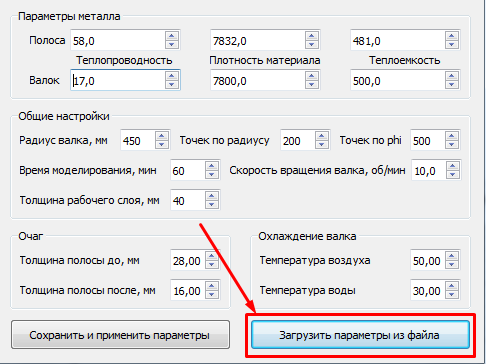
\includegraphics[width=0.9\linewidth]{20} \\} 
\end{minipage} 
\hfill 
\begin{minipage}[h]{0.49\linewidth} 
\center{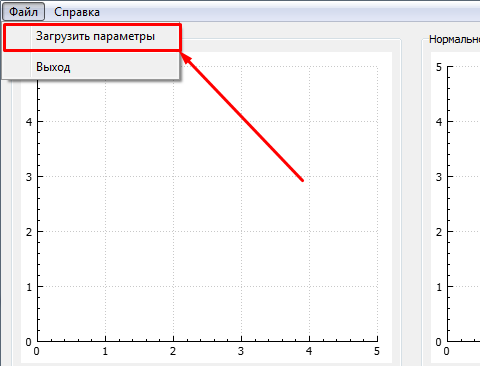
\includegraphics[width=0.9\linewidth]{21} \\ } 
\end{minipage} 
\caption{Кнопка для открытия окна с настройками} 
\end{figure}

Затем выбрать файл формата <<.hrp>>. Настройки автоматически сохранятся, соответственно дополнительно нажимать на кнопку <<Сохранить и применить параметры>> не нужно.

3) Основной расчет.

Чтобы выполнить эту функцию необходимо на главном экране нажать на кнопку <<Рассчитать температуру>>.
\blockschema{12}{Кнопка для основного расчета}

В течение нескольких секунд будет производиться расчет и вывод полученной информации на экран. Необходимо немного подождать завершения операции. В результате на экране появятся графики изменения самых важных величин (теплового потока, нормального и касательного напряжений, предела текучести и сопротивления деформации) по длине очага и график распределения тепла на выходе из очага. И, что самое главное, разностную сетку со значениями температуры в рабочем слое валка и в полосе.
\blockschema{15}{Главное окно после расчетов}

\subsubsection{Сообщения оператору}
В случае возникновения ошибок при работе с программой, не описанных ниже в данном разделе, необходимо обращаться к ответственному администратору.

\begin{itemize}
\item <<Настройки не загружены!>>
\fig{14}{Ошибка заполнения полей}
\end{itemize}

Такая ошибка может возникнуть из-за импорта настроек из файла с нарушенной структурой, либо с недостающими параметрами. Так же она может возникнуть из-за ошибочного ввода данных. Для исправления необходимо сохранить нужные параметры заново так, как описано в п. 3.2.3.

В качестве контрольного примера рекомендуется выполнить операции, описанные в п. 3.2.3. настоящего документа.

\newpage
%\section{Численное решение поставленной задачи}

В отличае от главы 2, в которой приводилось аналитическое решение рассматриваемой задачи, глава 4 должна содержать численное решение задачи с использованием разработанного и представленного в главе 3 программного обеспечения. Глава 4 может содержать оценку адекватности модели и метода ее решения, а также практические рекомендации специалистам предметной области по решению задачи и оценке полученных результатов.

Все главы выпускной квалификационной работы могут включать в графические элементы. Примеры рисунков и таблиц представлены в приложениях 1 и 2. 







%----------------------------------------------------------------------------------------
%	CONCLUSION
%----------------------------------------------------------------------------------------

%\newpage

\section*{Заключение} \addcontentsline{toc}{section}{Заключение}

В заключении подводятся основные итоги по работе (в соответствии с поставленными во введении целью и задачами).

%----------------------------------------------------------------------------------------
%	BIBLIOGRAPHY
%----------------------------------------------------------------------------------------

%\newpage
\renewcommand\refname{Список использованных источников}
\addcontentsline{toc}{section}{Список использованных источников}

\printbibliography

%----------------------------------------------------------------------------------------
%	APPENDIX
%----------------------------------------------------------------------------------------

%%\appendix
\newpage
\section*{} \addcontentsline{toc}{section}{Приложения}
\subsection*{}

\renewcommand{\thefigure}{A.\arabic{figure}}
\renewcommand{\thetable}{A.\arabic{table}}
\setcounter{table}{0}
\setcounter{figure}{0}   
\begin{center}
\textbf{Приложение А}

(рекомендуемое)

\end{center}


\begin{figure}[htbp]
	\label{primer_risunka}
	\begin{center}
		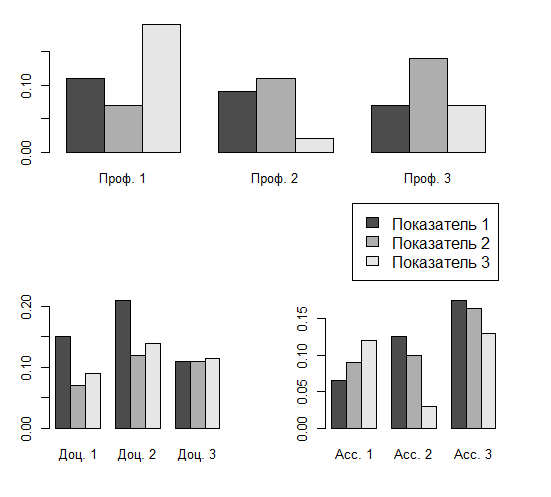
\includegraphics[scale=0.8]{Images/img1.png}
	\end{center}
	\caption{Пример рисунка}
\end{figure}

\newpage
\subsection*{}

\renewcommand{\thefigure}{Б.\arabic{figure}}
\renewcommand{\thetable}{Б.\arabic{table}}
\setcounter{table}{0}
\setcounter{figure}{0}
\begin{center}
\textbf{Приложение Б}

(рекомендуемое)

\end{center}

\noindent
\begin{table}[htbp]
	\caption{Название таблицы}
	\begin{tabularx}{\textwidth}{|X|X|X|X|X|}
		\hline 
		\multirow{2}{*}{Головка} 
		& \multicolumn{2}{c|}{Графа 1} & \multicolumn{2}{c|}{Графа 2} \\
		\cline{2-5}
  		& Подграфа 1 & Подграфа 2 & Подграфа 3 & Подграфа 4 \\ 
		\hline
  		&   &   &   &  \\ 
		\hline
  		&   &   &   &  \\ 
		\hline 
	\end{tabularx}
\end{table}






\end{document} 